\documentclass[a4paper, oneside]{article}
\usepackage[utf8]{inputenc}
\usepackage[T1]{fontenc}
\usepackage{amssymb}
\usepackage[polish]{babel}
\usepackage{float}
\usepackage[table]{xcolor}
\usepackage{graphicx}

\let\endtitlepage\relax
\newcommand{\X}{\checkmark}

\title{\Large\textbf{Ćwiczenia z Sieci komputerowych\\ Lista 1}}
\author{Jakub Grobelny (300481)}
\date{}

\begin{document}

\begin{titlepage}
    \maketitle
\end{titlepage}

\begin{table}[H]
    \centering
    \begin{tabular}{|l|c|c|c|c|c|c|c|c|c|c|}
    \hline
    \textbf{Zadanie}    & 1 & 2 & 3 & 4 & 5 & 6 & 7 & 8 & 9 & 10 \\\hline
    \textbf{Rozwiązane} &\X &\X &\X &\X &\X &\X &\X &   &   &    \\\hline
\end{tabular}
\end{table}

\begin{description}
    \item[Zadanie 1.]$ $

    \begin{itemize}
        \item {
            \texttt{10.1.2.3/8}

            Prefiks ma 8 bitów, czyli adres sieci to pierwszy bajt i 
            same zera (\texttt{10.0.0.0/8}).
            
            Adres rozgłoszeniowy to \texttt{10.255.255.255/8}. 
            
            \texttt{10.1.2.3/8} \textbf{jest adresem komputera}.

            Przykładowy adres innego komputera: \texttt{10.1.2.4/8}.
        }

        \item {
            \texttt{156.17.0.0/16}

            Prefiks ma 16 bitów, czyli adres \textbf{jest adresem sieci} 
            \texttt{156.17.0.0/16} bo od szesnastego bitu są same zera.

            Adres rozgłoszeniowy: \texttt{156.17.255.255/16}

            Przykładowy adres komputera: \texttt{156.17.42.42/16}.
        }

        \item {
            \texttt{99.99.99.99/27}

            W postaci binarnej (podkreślony prefiks z 27 bitów): 

            \underline{\texttt{01100011 01100011 01100011 011}}\texttt{00011}

            Widać zatem, że \textbf{jest to adres komputera} (sufiks nie składa 
            się z samych zer ani z samych jedynek).

            Adres sieci to \texttt{99.99.99.96/27} (prefiks + 5 zer na końcu).

            Adres rozgłoszeniowy to \texttt{99.99.99.127/27} (prefiks + 5 
            jedynek na końcu).

            Przykładowy adres innego komputera: \texttt{99.99.99.100/27}
        }

        \item {
            \texttt{156.17.64.4/30}

            Binarnie: 
            \underline{\texttt{10011100 00010001 01000000 000001}}\texttt{00}

            Widać, że adres jest pierwszym o tym prefiksie, więc 
            \textbf{jest to adres sieci}.

            Adres rozgłoszeniowy: \texttt{156.17.64.7/30}.

            Przykładowy adres komputera: \texttt{156.17.64.6/30}.
        }

        \item {
            \texttt{123.123.123.123/32}

            Prefiks to wszystkie cztery bajty, więc 
            \textbf{jest to jeden konkretny adres komputera} a nie zakres 
            adresów (czyli adres sieci $=$ adres rozgłoszeniowy $=$ 
            adres komputera).
        }

    \end{itemize}
    \item[Zadanie 2.] {
        \texttt{10.10.0.0/16} $=$ 
        \underline{\texttt{00001010 00001010}} \texttt{00000000 00000000}.

        Żeby uzyskać 5 podsieci, musielibyśmy poświęcić dodatkowe 3 bity na 
        maskę podsieci. Przy użyciu trzech bitów można zakodować aż 8 różnych 
        wartości, więc 3 z nich by się zmarnowały.

        \textbf{Rozwiązanie}: dzielimy sieć na 4 podsieci, a 
        następnie jedną z tych podsieci dzielimy jeszcze na dwie, co da nam 
        łącznie pięć sieci.

        Dostajemy więc następujące podsieci:
        \begin{table}[H]
        \centering
        \begin{tabular}{|l|c|}
            \hline
            \textbf{Zakres adresów} & \textbf{Trzeci bajt adresu} \\\hline\hline
            \texttt{10.10.0.0/18}   & \underline{00}\texttt{000000} \\ \hline
            \texttt{10.10.64.0/18}  & \underline{01}\texttt{000000} \\ \hline
            \texttt{10.10.128.0/18} & \underline{10}\texttt{000000} \\ \hline
            \texttt{10.10.192.0/19} & \underline{110}\texttt{00000} \\ \hline
            \texttt{10.10.224.0/19} & \underline{111}\texttt{00000} \\ \hline
        \end{tabular}
        \end{table}

        Są one oczywiście rozłączne, a każdy adres z zakresu 
        \texttt{10.10.0.0/16} należy do którejś z nich.\\

        Sieć \texttt{10.10.0.0/16} miała 65536 możliwych adresów, z czego dwa z
        nich to adres sieci i adres rozgłoszeniowy (co daje 65534 adresy dla 
        komputerów).

        Po podzieleniu na pięć podsieci również mamy 65536 adresów, ale każda
        podsieć ma teraz swój własny adres sieci i adres rozgłoszeniowy, co 
        daje nam $65536 - 5 \cdot 2 = 65526$ adresów. \textbf{Straciliśmy więc 
        osiem możliwych adresów możliwych do użycia przy adresowaniu 
        komputerów}.\\

        \textbf{Pytanie}: jaki jest minimalny rozmiar podsieci, który możesz 
        uzyskać w ten sposób?
        
        \textbf{Odpowiedź}: minimalną podsieć możemy uzyskać poprzez podział
        polegający na dzieleniu najmniejszej z uzyskanych podsieci na dwie 
        kolejne. Taki podział wyglądałby następująco:

        \begin{table}[H]
        \centering
        \begin{tabular}{|l|c|}
        \hline
        \textbf{Zakres adresów} & \textbf{Trzeci bajt adresu} \\\hline\hline
        \texttt{10.10.0.0/17}  & \underline{\texttt{0}}\texttt{0000000}\\\hline
        \texttt{10.10.128.0/18}& \underline{\texttt{10}}\texttt{000000}\\\hline
        \texttt{10.10.192.0/19}& \underline{\texttt{110}}\texttt{00000}\\\hline
        \texttt{10.10.224.0/20}& \underline{\texttt{1110}}\texttt{0000}\\\hline
        \texttt{10.10.240.0/20}& \underline{\texttt{1111}}\texttt{0000}\\\hline
        \end{tabular}
        \end{table}

        Jak widać w tabeli, najmniejsze dwie podsieci mają jedynie $2^{12}=4096$
        możliwych adresów, czyli tylko 4094 adresów możliwych do użycia przy 
        adresowaniu komputerów.\\\\
    }
\\
    \item[Zadanie 3.] {
        Oryginalna tablica routingu:

        \begin{table}[H]
        \centering
        \begin{tabular}{|l|l|c|l|}
        \hline
            & \textbf{Adresy}     
            & \textbf{Dokąd wysłać} 
            & \textbf{Zakres adresów} \\ \hline \hline
        1   &  \texttt{0.0.0.0/0}
            & \cellcolor{blue!35}  router A 
            & \texttt{0.0.0.0} -- \texttt{255.255.255.255} \\ \hline
        2   & \texttt{10.0.0.0/23}   
            & \cellcolor{green!35} router B 
            & \texttt{10.0.0.0} -- \texttt{10.0.1.255} \\ \hline
        3   & \texttt{10.0.2.0/24}   
            & \cellcolor{green!35} router B 
            & \texttt{10.0.2.0} -- \texttt{10.0.2.255} \\ \hline
        4   & \texttt{10.0.3.0/24}   
            & \cellcolor{green!35} router B 
            & \texttt{10.0.3.0} -- \texttt{10.0.3.255} \\ \hline
        5   & \texttt{10.0.1.0/24}   
            & \cellcolor{red!35}   router C 
            & \texttt{10.0.1.0} -- \texttt{10.0.1.255} \\ \hline
        6   & \texttt{10.0.0.128/25} 
            & \cellcolor{green!35} router B 
            & \texttt{10.0.0.128} -- \texttt{10.0.0.255} \\ \hline
        7   &\texttt{10.0.1.8/29}   
            & \cellcolor{green!35} router B 
            & \texttt{10.0.1.8} -- \texttt{10.0.1.15} \\ \hline
        8   &\texttt{10.0.1.16/29}  
            & \cellcolor{green!35} router B 
            & \texttt{10.0.1.16} -- \texttt{10.0.1.23} \\ \hline
        9   &\texttt{10.0.1.24/29}  
            & \cellcolor{green!35} router B 
            & \texttt{10.0.1.24} -- \texttt{10.0.1.31} \\ \hline
        \end{tabular}
        \end{table}

        Wpisy 8 i 9 różnią się jedynie na ostatnim bicie prefiksu a ich 
        prefiksy są takiej samej długości. Możemy więc złączyć je w jeden zakres
        \texttt{10.0.1.16/28} z prefiksem krótszym o 1 bit.

        Tę samą metodę możemy zastosować do wpisów 3 i 4. Po złączeniu utworzą 
        one zakres \texttt{10.0.2.0/23}. Wówczas jednak możemy powtórzyć
        to samo dla nowego zakresu oraz 2. Różnią się jedynie dwudziestym
        trzecim (ostatnim) bitem prefiksu, więc można utworzyć większy
        zakres \texttt{10.0.0.0/22}.

        Widać również, że wpis 6, czyli \texttt{10.0.0.128/25}, jest
        podzbiorem nowo utworzonego \texttt{10.0.0.0/22}. Jednocześnie
        \texttt{10.0.0.128/25} jest rozłączny z \texttt{10.0.1.0/24}, więc
        możemy go usunąć.
        \\

        Po zmniejszeniu:

        \begin{table}[H]
        \centering
        \begin{tabular}{|l|l|c|l|}
        \hline
            & \textbf{Adresy}     
            & \textbf{Dokąd wysłać} 
            & \textbf{Zakres adresów} \\ \hline \hline
        1   &  \texttt{0.0.0.0/0}
            & \cellcolor{blue!35}  router A 
            & \texttt{0.0.0.0} -- \texttt{255.255.255.255} \\ \hline
        2*  & \texttt{10.0.0.0/22}   
            & \cellcolor{green!35} router B 
            & \texttt{10.0.0.0} -- \texttt{10.0.3.255} \\ \hline
        5   & \texttt{10.0.1.0/24}   
            & \cellcolor{red!35}   router C 
            & \texttt{10.0.1.0} -- \texttt{10.0.1.255} \\ \hline
        8*  &\texttt{10.0.1.16/28}  
            & \cellcolor{green!35} router B 
            & \texttt{10.0.1.16} -- \texttt{10.0.1.31} \\ \hline
        7   &\texttt{10.0.1.8/29}   
            & \cellcolor{green!35} router B 
            & \texttt{10.0.1.8} -- \texttt{10.0.1.15} \\ \hline

        \end{tabular}
        \end{table}
    }

    \item[Zadanie 4.] {
        Oryginalna tablica routingu:

        \begin{table}[H]
        \centering
        \begin{tabular}{|l|l|c|l|}
        \hline
            & \textbf{Adresy}     
            & \textbf{Dokąd wysłać} 
            & \textbf{Zakres adresów} \\ \hline \hline
        1   & \texttt{0.0.0.0/0}
            & \cellcolor{blue!35} router A 
            & \texttt{0.0.0.0} -- \texttt{255.255.255.255} \\ \hline
        2   & \texttt{10.0.0.0/8}
            & \cellcolor{green!35} router B
            & \texttt{10.0.0.0} -- \texttt{10.255.255.255} \\ \hline
        3   & \texttt{10.3.0.0/24}
            & \cellcolor{red!35} router C
            & \texttt{10.3.0.0} -- \texttt{10.3.0.255} \\ \hline
        4   & \texttt{10.3.0.32/27}
            & \cellcolor{green!35} router B
            & \texttt{10.3.0.32} -- \texttt{10.3.0.63} \\ \hline
        5   & \texttt{10.3.0.64/27}
            & \cellcolor{green!35} router B
            & \texttt{10.3.0.64} -- \texttt{10.3.0.95} \\ \hline
        6   & \texttt{10.3.0.96/27}
            & \cellcolor{green!35} router B
            & \texttt{10.3.0.96} -- \texttt{10.3.0.127} \\ \hline
        \end{tabular}
        \end{table}

        Analogicznie do poprzedniego zadania, można zredukować 5 i 6
        do jednego wpisu \texttt{10.3.0.64/26} poprzez skrócenie prefiksu
        o bit.
    
        Zmniejszona tabela:\\
        
        \begin{table}[H]
        \centering
        \begin{tabular}{|l|l|c|l|}
        \hline
            & \textbf{Adresy}     
            & \textbf{Dokąd wysłać} 
            & \textbf{Zakres adresów} \\ \hline \hline
        1   & \texttt{0.0.0.0/0}
            & \cellcolor{blue!35} router A 
            & \texttt{0.0.0.0} -- \texttt{255.255.255.255} \\ \hline
        2   & \texttt{10.0.0.0/8}
            & \cellcolor{green!35} router B
            & \texttt{10.0.0.0} -- \texttt{10.255.255.255} \\ \hline
        3   & \texttt{10.3.0.0/24}
            & \cellcolor{red!35} router C
            & \texttt{10.3.0.0} -- \texttt{10.3.0.255} \\ \hline
        5*  & \texttt{10.3.0.64/26}
            & \cellcolor{green!35} router B
            & \texttt{10.3.0.64} -- \texttt{10.3.0.127} \\ \hline
        4   & \texttt{10.3.0.32/27}
            & \cellcolor{green!35} router B
            & \texttt{10.3.0.32} -- \texttt{10.3.0.63} \\ \hline
        \end{tabular}
        \end{table}

        Można jednak zauważyć, że gdybyśmy byli w stanie ,,wyciąć dziurę'' we
        wpisie 3, która miałaby zakres adresów od \texttt{10.3.0.32} do
        \texttt{10.3.0.128}, to wówczas można by usunąć wpisy 5* i 4, i zamiast 
        tego rozdzielić wpis 3 na dwa rozłączne.

        Przedstawiono to na poniższym obrazku:

        \begin{figure}[H]
            \centering
            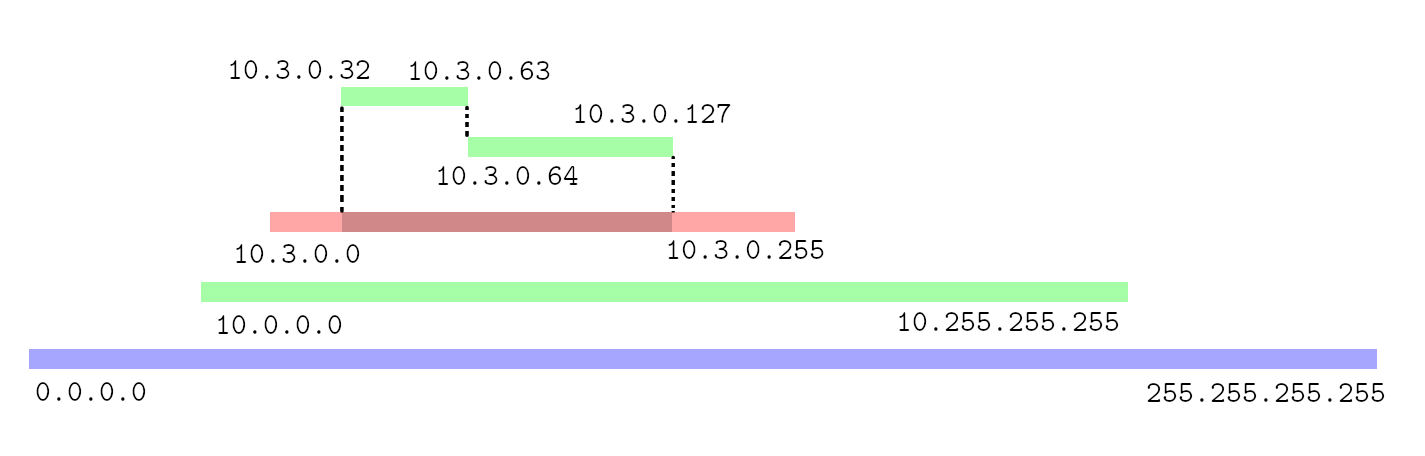
\includegraphics[scale=1.25]{zad4.png}
        \end{figure}
        
        Można podzielić 3 na \texttt{10.3.0.0/27} (zakres 
        \texttt{10.3.0.0} -- \texttt{10.3.0.31}) i na 
        \texttt{10.3.0.128/25} (zakres \texttt{10.3.0.128} 
        -- \texttt{10.3.0.255}).

        Teraz możemy usunąć wpisy 5* i 4, gdyż sprawdzany adres może po prostu
        ,,wpaść'' w powstałą ,,dziurę'' i dopasować się do wpisu 2, który tak jak 5* i 4 kieruje do routera B.

        Daje to nam ostateczną tabelę:

        \begin{table}[H]
        \centering
        \begin{tabular}{|l|l|c|l|}
        \hline
            & \textbf{Adresy}     
            & \textbf{Dokąd wysłać} 
            & \textbf{Zakres adresów} \\ \hline \hline
        1   & \texttt{0.0.0.0/0}
            & \cellcolor{blue!35} router A 
            & \texttt{0.0.0.0} -- \texttt{255.255.255.255} \\ \hline
        2   & \texttt{10.0.0.0/8}
            & \cellcolor{green!35} router B
            & \texttt{10.0.0.0} -- \texttt{10.255.255.255} \\ \hline
        3*  & \texttt{10.3.0.0/27}
            & \cellcolor{red!35} router C
            & \texttt{10.3.0.0} -- \texttt{10.3.0.31} \\ \hline
        3** & \texttt{10.3.0.128/25}
            & \cellcolor{red!35} router C
            & \texttt{10.3.0.128} -- \texttt{10.3.0.255} \\ \hline
        \end{tabular}
        \end{table}
    }

    \item [Zadanie 5.]$ $

    \begin{description}
        \item [Teza.] {
            Aby zasada najlepszego dopasowania odpowiadała wyborowi ,,pierwszy
            pasujący'', należy uporządkować wpisy malejąco względem długości 
            prefiksów.
        }
        \item [Dowód.] {
            Załóżmy, że wpisy są posortowane malejąco względem długości
            prefiksów. Pokażemy, że wybór pierwszego pasującego wpisu
            prowadzi do najlepszego dopasowania.\\

            Niech $i$ będzie dowolnym adresem IP i
            niech $k$ będzie pierwszym w kolejności rozpatrywania wpisem w 
            tablicy routingu, do którego można dopasować $i$.

            Niech $n$ będzie długością prefiksu $k$. Oznacza to, że
            pierwsze $n$ bitów $i$ jest identyczne z prefiksem $k$.

            Weźmy dowolny wpis $l$ występujący w tablicy za $k$.
            Z założenia, że wpisy posortowane są malejąco względem 
            długości prefiksów, wiemy, że długość $m$ prefiksu $l$
            spełnia nierówność $m \leq n$. Oznacza to, że dopasowane
            zostanie nie więcej bitów adresu $i$ niż $n$, czyli $k$
            jest nie gorszym dopasowaniem niż $l$, więc wybór
            ,,pierwszego pasującego'' odpowiada zasadzie najlepszego
            dopasowania, co należało udowodnić.
        }
        
    \end{description}

    \item[Zadanie 6.]$ $
    \begin{figure}[H]
        \centering
        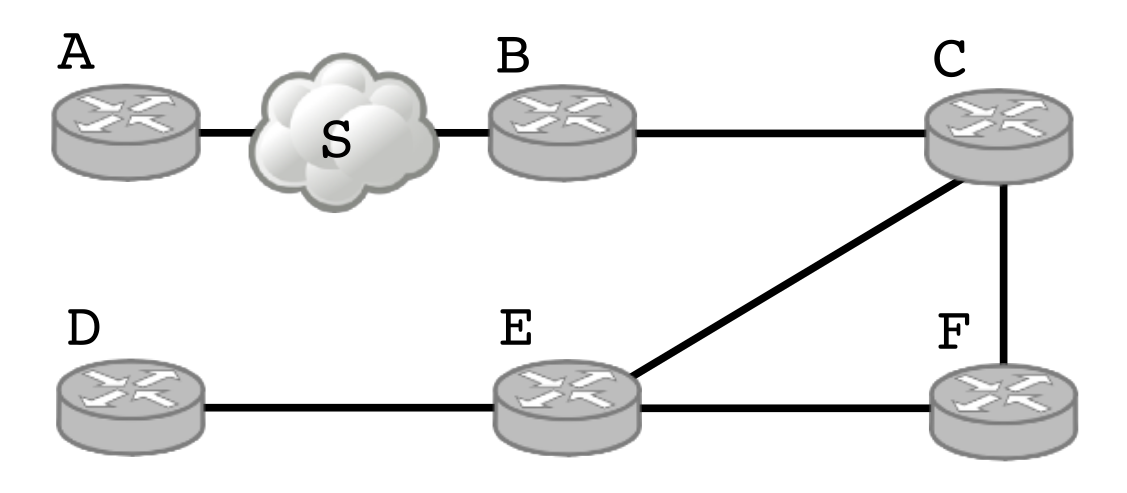
\includegraphics[scale=0.25]{zad6.png}
    \end{figure}

    Algorytm działa w taki sposób, że sąsiadujące routery co jakiś
    czas przekazują sobie swoje tablice routingu. Na ich podstawie 
    routery wyznaczają najkrótsze ścieżki metodą relaksacji.

    Początkowy stan (każdy zna tylko swoich sąsiadów, puste komórki oznaczają,
    że droga nie jest znana (długość wynosi nieskończoność)):
    \begin{table}[H]
    \centering
    \begin{tabular}{|l|c|c|c|c|c|c|}
    \hline
    & \textbf{A} & \textbf{B} 
    & \textbf{C} & \textbf{D} 
    & \textbf{E} & \textbf{F} \\ \hline\hline
    trasa do A & - & 1 &   &   &   &   \\ \hline
    trasa do B & 1 & - & 1 &   &   &   \\ \hline
    trasa do C &   & 1 & - &   & 1 & 1 \\ \hline
    trasa do D &   &   &   & - & 1 &   \\ \hline
    trasa do E &   &   & 1 & 1 & - & 1 \\ \hline
    trasa do F &   &   & 1 &   & 1 & - \\ \hline
    trasa do S & 1 & 1 &   &   &   &   \\ \hline
    \end{tabular}
    \end{table}

    \begin{table}[H]
    \centering
    \begin{tabular}{|l|c|c|c|c|c|c|}
    \hline
    & \textbf{A} & \textbf{B} 
    & \textbf{C} & \textbf{D} 
    & \textbf{E} & \textbf{F} \\ \hline\hline
    trasa do A & -         & 1         & 2 \cellcolor{green!10}(od B) &           &           &   
    \\ \hline
    trasa do B & 1         & -         & 1         &           & 2 \cellcolor{green!10}(od C) & 2 \cellcolor{green!10}(od C) 
    \\ \hline
    trasa do C & 2 \cellcolor{green!10}(od B) & 1         & -         & 2 \cellcolor{green!10}(od E) & 1         & 1 
    \\ \hline
    trasa do D &           &           & 2 \cellcolor{green!10}(od E) & -         & 1         & 2 \cellcolor{green!10}(od E) 
    \\ \hline
    trasa do E &           & 2 \cellcolor{green!10}(od C) & 1         & 1         & -         & 1 
    \\ \hline
    trasa do F &           & 2 \cellcolor{green!10}(od C) & 1         & 2 \cellcolor{green!10}(od E) & 1         & - 
    \\ \hline
    trasa do S & 1         & 1         & 2 \cellcolor{green!10}(od B) &           &           &   
    \\ \hline
    \end{tabular}
    \end{table}

    \begin{table}[H]
    \centering
    \begin{tabular}{|l|c|c|c|c|c|c|}
    \hline
    & \textbf{A} & \textbf{B} 
    & \textbf{C} & \textbf{D} 
    & \textbf{E} & \textbf{F} \\ \hline\hline
    trasa do A & -         & 1         & 2 (B)    &           & 3 \cellcolor{green!10}(od C) & 3 \cellcolor{green!10}(od C) \\ \hline
    trasa do B & 1         & -         & 1         & 3 \cellcolor{green!10}(od E) & 2 (C)       & 2 (C)      \\ \hline
    trasa do C & 2 (B)     & 1         & -         & 2   (E)    & 1         & 1         \\ \hline
    trasa do D &           & 3 \cellcolor{green!10}(od C) & 2  (E)     & -         & 1         & 2   (E)    \\ \hline
    trasa do E & 3 \cellcolor{green!10}(od B) & 2 (C)      & 1         & 1         & -         & 1         \\ \hline
    trasa do F & 3 \cellcolor{green!10}(od B) & 2 (C)      & 1         & 2 (E)      & 1         & -         \\ \hline
    trasa do S & 1         & 1         & 2    (B)  &           & 3 \cellcolor{green!10}(od C) & 3 \cellcolor{green!10}(od C) \\ \hline
    \end{tabular}
    \end{table}

    \begin{table}[H]
    \centering
    \begin{tabular}{|l|c|c|c|c|c|c|}
    \hline
    & \textbf{A} & \textbf{B} 
    & \textbf{C} & \textbf{D} 
    & \textbf{E} & \textbf{F} \\ \hline\hline
    trasa do A & -        & 1     & 2 (B) & 4 \cellcolor{green!10}(od E) & 3 (C) & 3 (C) \\ \hline
    trasa do B & 1        & -     & 1     & 3 (E)    & 2 (C) & 2 (C) \\ \hline
    trasa do C & 2 (B)    & 1     & -     & 2 (E)    & 1     & 1     \\ \hline
    trasa do D & 4 \cellcolor{green!10}(od B) & 3 (C) & 2 (E) & -        & 1     & 2 (E) \\ \hline
    trasa do E & 3 (B)    & 2 (C) & 1     & 1        & -     & 1     \\ \hline
    trasa do F & 3 (B)    & 2 (C) & 1     & 2 (E)    & 1     & -     \\ \hline
    trasa do S & 1        & 1     & 2 (B) & 4 \cellcolor{green!10}(od E) & 3 (C) & 3 (C) \\ \hline
    \end{tabular}
    \end{table}

    Ostatecznie dostajemy następujące długości dróg:

    \begin{table}[H]
    \centering
    \begin{tabular}{|l|c|c|c|c|c|c|}
    \hline
    & \textbf{A} & \textbf{B} 
    & \textbf{C} & \textbf{D} 
    & \textbf{E} & \textbf{F} \\ \hline\hline
    trasa do A & -     & 1     & 2 (B) & 4 (E) & 3 (C) & 3 (C) \\ \hline
    trasa do B & 1     & -     & 1     & 3 (E) & 2 (C) & 2 (C) \\ \hline
    trasa do C & 2 (B) & 1     & -     & 2 (E) & 1     & 1     \\ \hline
    trasa do D & 4 (B) & 3 (C) & 2 (E) & -     & 1     & 2 (E) \\ \hline
    trasa do E & 3 (B) & 2 (C) & 1     & 1     & -     & 1     \\ \hline
    trasa do F & 3 (B) & 2 (C) & 1     & 2 (E) & 1     & -     \\ \hline
    trasa do S & 1     & 1     & 2 (B) & 4 (E) & 3 (C) & 3 (C) \\ \hline
    \end{tabular}
    \end{table}
    
    Jak widać wszystkie routery znają już drogi do wszystkich innych routerów.
    Można również sprawdzić, że wyznaczone drogi są najkrótszymi w tej sieci,
    co oznacza, że \textbf{stan stabilny został osiągnięty w trzech krokach}.

    \item [Zadanie 7.] {
        Rozpatrujemy teraz sytuację, w której po utworzeniu tablicy z
        zadania 6 dodane zostaje nowe połączenie (pomiędzy \texttt{A} 
        i \texttt{D}). Nasza sieć wygląda zatem tak:

        \begin{figure}[H]
            \centering
            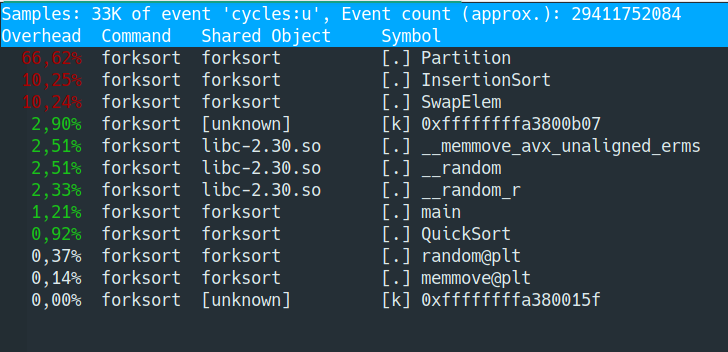
\includegraphics[scale=0.25]{zad7.png}
        \end{figure}

        W zerowym kroku routery \texttt{A} i \texttt{D} muszą się o sobie
        dowiedzieć. Mamy zatem następującą tablicę:

        \begin{table}[H]
        \centering
        \begin{tabular}{|l|c|c|c|c|c|c|}
        \hline
        & \textbf{A} & \textbf{B} 
        & \textbf{C} & \textbf{D} 
        & \textbf{E} & \textbf{F} \\ \hline\hline
        trasa do A & -     & 1     & 2 (B) & 1 \cellcolor{green!10}(nowa z A) & 3 (C) & 3 (C) \\ \hline
        trasa do B & 1     & -     & 1     & 3 (E) & 2 (C) & 2 (C) \\ \hline
        trasa do C & 2 (B) & 1     & -     & 2 (E) & 1     & 1     \\ \hline
        trasa do D & 1 \cellcolor{green!10}(nowa z D) & 3 (C) & 2 (E) & -     & 1     & 2 (E) \\ \hline
        trasa do E & 3 (B) & 2 (C) & 1     & 1     & -     & 1     \\ \hline
        trasa do F & 3 (B) & 2 (C) & 1     & 2 (E) & 1     & -     \\ \hline
        trasa do S & 1     & 1     & 2 (B) & 4 (E) & 3 (C) & 3 (C) \\ \hline
        \end{tabular}
        \end{table}

        Teraz gdy routery zaczną wymieniać się swoimi tablicami, część
        z nich będzie mogła skrócić znane sobie ścieżki.

        \begin{table}[H]
        \centering
        \begin{tabular}{|l|c|c|c|c|c|c|}
        \hline
        & \textbf{A} & \textbf{B} 
        & \textbf{C} & \textbf{D} 
        & \textbf{E} & \textbf{F} \\ \hline\hline
        trasa do A & -        & 1     & 2 (B) & 1         & \cellcolor{green!10} 2 \cellcolor{green!10}(od D) & 3 (C) \\ \hline
        trasa do B & 1        & -     & 1     & 2 \cellcolor{green!10}(od A)  & 2 (C) & 2 (C) \\ \hline
        trasa do C & 2 (B)    & 1     & -     & 2 (E)     & 1     & 1     \\ \hline
        trasa do D & 1   & 2 \cellcolor{green!10}(od A) & 2 (E) & -           & 1     & 2 (E) \\ \hline
        trasa do E & 2 \cellcolor{green!10}(od D) & 2 (C) & 1     & 1         & -     & 1     \\ \hline
        trasa do F & 3 (B)    & 2 (C) & 1     & 2 (E)     & 1     & -     \\ \hline
        trasa do S & 1        & 1     & 2 (B) & 2 \cellcolor{green!10}(od A)  & 3 (C) & 3 (C) \\ \hline
        \end{tabular}
        \end{table}

        Ostatecznie dostajemy więc następującą tablicę:
        \begin{table}[H]
        \centering
        \begin{tabular}{|l|c|c|c|c|c|c|}
        \hline
        & \textbf{A} & \textbf{B} 
        & \textbf{C} & \textbf{D} 
        & \textbf{E} & \textbf{F} \\ \hline\hline
        trasa do A & -        & 1     & 2 (B) & 1         & 2 (D) & 3 (C) \\ \hline
        trasa do B & 1        & -     & 1     & 2 (A)  & 2 (C) & 2 (C) \\ \hline
        trasa do C & 2 (B)    & 1     & -     & 2 (E)     & 1     & 1     \\ \hline
        trasa do D & 1   & 2 (A) & 2 (E) & -           & 1     & 2 (E) \\ \hline
        trasa do E & 2 (D) & 2 (C) & 1     & 1         & -     & 1     \\ \hline
        trasa do F & 3 (B)    & 2 (C) & 1     & 2 (E)     & 1     & -     \\ \hline
        trasa do S & 1        & 1     & 2 (B) & 2 (A)  & 3 (C) & 3 (C) \\ \hline
        \end{tabular}
        \end{table}

        W tym momencie znów osiągnięto stan stabilny, bo wszystkie ścieżki
        są już najkrótsze i nic nie będzie się zmieniać.
    }
\end{description}

\end{document}

